
\documentclass[10pt]{beamer}
% \usepackage{subfiles}

\usepackage[danish]{babel}
\usepackage[utf8]{inputenc}
\usetheme[progressbar=frametitle]{metropolis}
\usepackage{appendixnumberbeamer}


\usepackage{booktabs}
\usepackage[scale=2]{ccicons}

% \usepackage{pgfplots}
% \usepgfplotslibrary{dateplot}

\definecolor{Orange}{RGB}{229,134,25}

\usepackage{xspace}
\newcommand{\themename}{\textbf{\textsc{metropolis}}\xspace}
\usepackage{listings}


\definecolor{background}{RGB}{226, 226, 226}


\lstset{ 
literate=% 
{Ö}{{\"O}}1 
{Ä}{{\"A}}1 
{Ü}{{\"U}}1 
{ß}{{\ss}}{ 1\negmedspace\,} 
{ü}{{\"u}}1 
{ä}{{\"a}}1 
{ö}{{\"o}}1 
{ø}{{\o}}{1\negmedspace\,} 
{Ø}{{\O}}{1\negthinspace\,\,} 
{å}{{\aa}}{1\negthickspace\,} 
{Å}{{\AA}}{1\negthinspace\;} 
{æ}{{\ae}}{1\negthinspace\;} 
{Æ}{{\AE}}{1\,\,}}

\lstdefinestyle{terminal}{
	language=bash,
	aboveskip=2mm,
	belowskip=2mm,
	showstringspaces=false,
	columns=flexible,
	basicstyle={\small\ttfamily},
	numbers=none,
	numberstyle=\footnotesize,
	commentstyle=\color{black},
	frame=single,
	framesep=2pt,
	breaklines=true,
	breakatwhitespace=false,
	backgroundcolor = \color{background},
	tabsize=2
}


\lstdefinestyle{python}{
	language=Python,
	aboveskip=2mm,
	belowskip=1mm,
	showstringspaces=false,
	columns=flexible,
	numbers=none,
	numberstyle=\footnotesize,
	commentstyle=\ttfamily\color{black},
	frame=single,
	framesep=2pt,
	breaklines=true,
	breakatwhitespace=false,
	backgroundcolor = \color{background},
	tabsize=2
}



\title{Lær Python dag 1 - modul 1}
\subtitle{Introduktion, basis python}
% \date{\today}
\date{}
\author{Steffen Berg Klenow \\Jonas Bamse Andersen}
\institute{Syddansk Universitet}
% \titlegraphic{\hfill
\includegraphics[height=1.5cm]{logo.pdf}}


\title{Lær Python dag 3 - modul 1}
\subtitle{Dictionaries og Filer}

\begin{document}

\maketitle

\begin{frame}{Indhold}
  \setbeamertemplate{section in toc}[sections numbered]
  \tableofcontents[hideallsubsections]
\end{frame}

\section{Recap}
\begin{frame}[fragile]{Hvad lærte I sidst?}
	Diskutér to minutter med sidemanden, hvad I lærte sidst.
	
	\begin{itemize}
		\item Hvad er en løkke?
		\item Hvad er en liste?
		\item Hvad kan vi med strenge?
		\item Andet?
	\end{itemize}
\end{frame}

%
%\begin{frame}[fragile]{Objekter og metoder}
%	I har prøvet at bruge funktioner som:
%	
%	\begin{lstlisting}[style=python]
%x = [1, 2]
%x.append(3)
%print(x)
%	\end{lstlisting}
%	
%	\pause
%	
%	Output:
%	\begin{lstlisting}[style=python]
%[1, 2, 3]
%	\end{lstlisting}
%	
%	\pause
%	
%	Har I undret jer over hvad punktummet betyder? \pause Hvorfor skriver man ikke:
%	\begin{lstlisting}[style=python]
%append(x, 3)
%	\end{lstlisting}
%	
%\end{frame}
%
%
%\begin{frame}[fragile]{Objekter og metoder}
%	Hvad sker der hvis man skriver:
%	
%	\begin{lstlisting}[style=python]
%x = 2
%x.append(3)
%	\end{lstlisting}
%	
%	\pause
%	
%	Output:
%	\begin{lstlisting}[style=python]
%...
% 
%AttributeError: 'int' object has no attribute 'append'
%	\end{lstlisting}
%	
%	\pause
%	
%	Men så må det være tilfældet at - \texttt{'list' object has attribute 'append'}.
%	
%	Hvad end det så betyder.
%	
%\end{frame}
%
%
%\begin{frame}[fragile]{Objekter og metoder}
%	Man kan tænke på det som et "interface" på "kassen".
%	
%	\begin{columns}
%		\column{0.4\textwidth}
%		\begin{lstlisting}[style=python]
%x = [1,2]
%x.append(3)
%		\end{lstlisting}
%		
%		\column{0.4\textwidth}
%		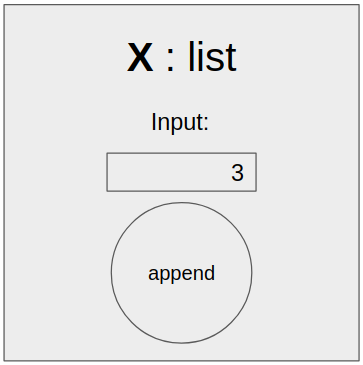
\includegraphics[width=0.8\textwidth]{objectmethod.png}
%	\end{columns}
%	
%	Eksempler på flere metoder kan findes på: \url{https://docs.python.org/3/tutorial/datastructures.html}
%\end{frame}
%
%
%\begin{frame}[fragile]{Objekter og metoder}
%Et andet eksempel kunne være
%
%\begin{columns}
%	\column{0.4\textwidth}
%	\begin{lstlisting}[style=python]
%x = "TEKST"
%x.lower()
%	\end{lstlisting}
%	
%	\column{0.4\textwidth}
%	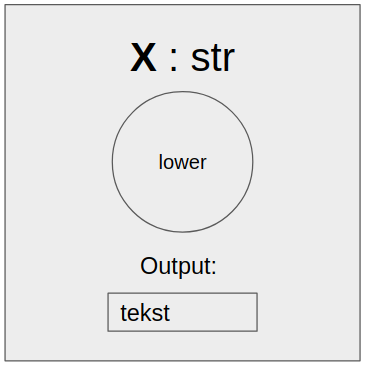
\includegraphics[width=0.8\textwidth]{stringmethod.png}
%\end{columns}
%
%Eksempler på flere metoder kan findes på: \url{https://docs.python.org/3/library/stdtypes.html#str}
%\end{frame}
%



\section{Dictionaries}

\begin{frame}[fragile]{Dictionaries - Gem data og find det igen}
	Navnet dictionary kommer tydeligvis fra det engelske ord for ordbog, og grunden til det er at man bruger et ord til at slå op med (key) for at finde en bestemt værdi (value). 
	
	\pause
	
	I de lister vi har set på bruges et bestemt tal (indeks) til at finde en bestemt værdi (value), dvs. værdierne har en bestemt rækkefølge.
	
	\pause
	
	Dictionaries minder meget om, men vi ved ikke noget om rækkefølgen på samme måde, tilgengæld slipper vi for at holde styr på, hvilken placering en værdi har.
	\pause
	
	I Python er "\{\}" og ":" vigtige for at lave et dictionary.
	
	Her er et eksempel på en dansk--engelsk ordbog over nogle dyr.
	\begin{lstlisting}[style=python]
translate = {"hund" : "dog", "kat" : "cat", "hest" : "horse"}
	\end{lstlisting}
\end{frame}

\begin{frame}[fragile]{Dictionaries - Gem data og find det igen}
Dictionary strukturen kan bruges til rigtig mange ting, f.eks.:

\medskip

\pause

\begin{columns}
	\column{0.5\textwidth}
	En person
	\begin{lstlisting}[style=python]
person = {"name"  : "Bamse",
          "age"   : 25,
          "height": 187}
	\end{lstlisting}
	
	\pause
	
	\column{0.45\textwidth}
	Et varekatalog
	\begin{lstlisting}[style=python]
price = {"Banana" : 10,
         "Milk"   : 5,
         "Bread"  : 20,
         "Salt"   : 2}
	\end{lstlisting}
\end{columns}	

\end{frame}

\begin{frame}[fragile]{Dictionaries - Gem data og find det igen}
	Lad os vende tilbage til ordbogseksemplet.

	Vi bruge vores dictionary til at slå oversættelserne op. Hvis man har et par "x" : "y", så bruger man den forreste streng, "x", som index for at finde "y".
	\begin{columns}
		\column{0.5\textwidth}
		\begin{lstlisting}[style=python]
translate = {"hund" : "dog", 
             "kat" : "cat", 
             "hest" : "horse"}
print(translate["hest"])
		\end{lstlisting}
		
		\pause
		\column{0.3\textwidth}
		\begin{lstlisting}[style=python]
horse
		\end{lstlisting}
	\end{columns}	
\end{frame}

\begin{frame}[fragile]{Dictionaries - Gem data og find det igen}
	Vi kan nemt tilføje nye dyr til vores ordbog.
	\begin{columns}
		\column{0.5\textwidth}
		\begin{lstlisting}[style=python]
translate = {"hund" : "dog", 
             "kat" : "cat", 
             "hest" : "horse"}
translate["ged"] = "goat"
translate["gris"] = "pig"
print(translate["ged"])
		\end{lstlisting}
		
		\pause
		\column{0.3\textwidth}
		\begin{lstlisting}[style=python]
goat
		\end{lstlisting}
	\end{columns}	
\end{frame}

\begin{frame}[fragile]{Dictionaries - Gem data og find det igen}
	Hvad sker der hvis vi vil oversætte noget vi ikke har i vores ordbog?
	\begin{columns}
		\column{0.5\textwidth}
		\begin{lstlisting}[style=python]
translate = {"hund" : "dog", 
             "kat" : "cat", 
             "hest" : "horse"}
print(translate["hamster"])
		\end{lstlisting}
		
		\pause
		\column{0.4\textwidth}
		\begin{lstlisting}[style=python]
KeyError                                  Traceback (most recent call last)
<ipython-input-20-55577e0fe5a3> in <module>()
----> 1 print(translate["hamster"])

KeyError: 'hamster'
		\end{lstlisting}
	\end{columns}	
\end{frame}


\begin{frame}[fragile]{Dictionaries - Gem data og find det igen}
	Heldigvis kan vi tjekke om en værdi findes i vores dictionary.
	\begin{columns}
		\column{0.5\textwidth}
		\begin{lstlisting}[style=python]
translate = {"hund" : "dog", 
             "kat" : "cat", 
             "hest" : "horse"}
def safeTranslate(animal):
  if (animal in translate):
    print(translate[animal])
  else:
    print("<" + animal + 
          "> not found")
		
safeTranslate("hamster")
safeTranslate("hund")
		\end{lstlisting}

		\pause
		\column{0.4\textwidth}
		\begin{lstlisting}[style=python]
<hamster> not found
dog
		\end{lstlisting}
	\end{columns}	
\end{frame}

\begin{frame}[fragile]{Dictionaries - Gem data og find det igen}
	Hvis vi skal løbe igennem alle ting i listen kan vi gøre det på flere forskellige måder.
	\begin{columns}
		\column{0.5\textwidth}
		\begin{lstlisting}[style=python]
translate = {"hund" : "dog", 
             "kat" : "cat", 
             "hest" : "horse"}
for navn in translate:
  print("Dansk:"
        , navn 
        , "Engelsk:"
        , translate[navn])
		\end{lstlisting}
		
		\pause
		\column{0.45\textwidth}
		\begin{lstlisting}[style=python]
Dansk: hund Engelsk: dog
Dansk: kat Engelsk: cat
Dansk: hest Engelsk: horse
		\end{lstlisting}
	\end{columns}	
\end{frame}

\begin{frame}[fragile]{Dictionaries - Gem data og find det igen}
	I stedet for at skulle "slå op" i vores ordbog i hvert gennemløb af loopet, kan vi få key - value parret direkte ved at bruge \texttt{.items()} på dictionariet.
	\begin{columns}
		\column{0.55\textwidth}
		\begin{lstlisting}[style=python]
translate = {"hund" : "dog", 
             "kat" : "cat", 
             "hest" : "horse"}
print(translate.items())
		\end{lstlisting}
		
		\pause
		\column{0.44\textwidth}
		\begin{lstlisting}[style=python]
dict_items([
	('hund', 'dog'), 
	('kat', 'cat'), 
	('hest', 'horse')])
		\end{lstlisting}
	\end{columns}	
\end{frame}

\begin{frame}[fragile]{Dictionaries - Gem data og find det igen}
	Vi kan også gøre det i et loop, hvor vi får værdierne direkte ud:
	\begin{columns}
		\column{0.55\textwidth}
		\begin{lstlisting}[style=python]
translate = {"hund" : "dog", 
             "kat" : "cat", 
             "hest" : "horse"}
for key, val in translate.items():
  print("Dansk:"
        , key
        , "Engelsk:"
        , val)
		\end{lstlisting}
		
		\pause
		\column{0.44\textwidth}
		\begin{lstlisting}[style=python]
Dansk: hund Engelsk: dog
Dansk: kat Engelsk: cat
Dansk: hest Engelsk: horse
		\end{lstlisting}
	\end{columns}	
\end{frame}

\begin{frame}[fragile]{Dictionaries - Gem data og find det igen}
	Lad os se, hvordan vi kan bruge de andre eksempler på dictionaries, vi havde fra starten.
	
	\begin{columns}
		\column{0.5\textwidth}
		\begin{lstlisting}[style=python]
person = {"name" : "Bamse",
          "age": 25,
          "height": 187}

if (person["height"] >= 180):
  print("You are tall", 
         person["name"])
else:
  print("You can still grow"
        , person["name"])
		\end{lstlisting}
		
		\pause
		\column{0.35\textwidth}
		\begin{lstlisting}[style=python]
You are tall Bamse
		\end{lstlisting}
	\end{columns}	
\end{frame}

\begin{frame}[fragile]{Dictionaries - Gem data og find det igen}
	Et andet eksempel kan være et dictionary som holder styr på varers priser i en butik.
	\begin{columns}
		\column{0.5\textwidth}
		\begin{lstlisting}[style=python]
price = {"Banana" : 10,
         "Milk" : 5,
         "Bread" : 20,
         "Salt" : 2}
print(price["Banana"])
		\end{lstlisting}
		
		\pause
		\column{0.3\textwidth}
		\begin{lstlisting}[style=python]
10
		\end{lstlisting}
	\end{columns}	
\end{frame}

\begin{frame}[fragile]{Dictionaries - Gem data og find det igen}
	Hvis vi tidligere ville have lavet et program der skulle tælle bogstaver i en lang streng, hvordan ville vi så have gjort?
	\pause
	
	Her er et forslag:
	\begin{lstlisting}[style=python]
s = "Lorem ipsum dolor sit amet..."
counts = [0] * 26	# [0,0,0,0,...]
for c in s.lower():
  if c == "a":
    counts[0] = counts[0] + 1
  elif c == "b":
    counts[1] = counts[1] + 1
  elif ...
.
.
.
	\end{lstlisting}
\end{frame}


\begin{frame}[fragile]{Dictionaries - Gem data og find det igen}
	Man kunne også gøre mange andre smartere ting end det, men det smarteste er nok at bruge dictionaries.
	\pause
	\begin{lstlisting}[style=python]
s = "fem flade flødeboller på et fladt flødebollefad"
d = {}
for c in s:
  if c not in d:
    d[c] = 0
  d[c] = d[c] + 1
print(d)
	\end{lstlisting}
\end{frame}

\begin{frame}[fragile]{Strenge og Dictionaries - Sidste bemærkninger}
	Som altid har jeg kun vist jer et lillebitte udsnit af hvilke funktioner der findes. Så husk, Google er kun få klik væk.
\end{frame}


%	\begin{lstlisting}[style=python]
%dyr = {"hund" : "dog", "kat" : "cat", "hest" : "horse", 
%"gris" : "pig", "ko" : "cow"}
%\end{lstlisting}


\section{Filer}

\begin{frame}{Filer og programmering}
	Filer bruges grundlæggende til to ting:
	\begin{itemize}
		\item Input til program (f.eks. til databehandling)
		\item Gemme output fra program (resultater, logs, \ldots)
	\end{itemize}
\end{frame}

\begin{frame}[fragile]{Åben/luk en fil}
	Vi åbner en fil med metoden \texttt{open()} som returnerer et filobjekt:
	\begin{lstlisting}[style=python]
f = open(<file>, <mode>)
	\end{lstlisting}
	
	\pause
	\texttt{open} tager parametrene \texttt{file} og \texttt{mode}:
	\begin{itemize}
		\item File: Stien til den fil som skal åbnes (string).
		\item Mode: Hvordan skal filen bruges 
		\begin{itemize}
			\item "r" for at læse (read)
			\item "w" for at skrive (write)
			\item "r+" for begge dele
			\item "a" for at lægge til (append)
		\end{itemize}
	\end{itemize}

\pause
	Når man er færdig med filen er det god stil at lukke den:
	\begin{lstlisting}[style=python]
f.close()
	\end{lstlisting}
\end{frame}


\begin{frame}[fragile]{Skriv til en fil}
Skriv til filen \texttt{hello.txt} på følgende vis:

\begin{lstlisting}[style=python]
f = open("hello.txt", "w")
f.write("Hello World!")
f.close()
\end{lstlisting}

Hvis vi skriver til en fil som ikke eksisterer oprettes en ny.

\end{frame}

\begin{frame}[fragile]{Skriv til en fil}
Vi skal selv indsætte vores linjeskift.

\begin{lstlisting}[style=python]
f = open("hello.txt", "w")
f.write("Lær python!!!\n")
f.write("IMADA SDU")
f.close()
\end{lstlisting}

Hvordan mon vores fil ser ud nu?

\pause

"w" overskriver filen uden at stille spørgsmål.

"a" bruges til at tilføje til en fil.

\end{frame}


\begin{frame}[fragile]{Læs fra en fil}
	Vi kan læse filen \texttt{hello.txt} på følgende vis:
	\begin{lstlisting}[style=python]
f = open("hello.txt", "r")
print(f.read())
f.close()
	\end{lstlisting}
	
\end{frame}

\begin{frame}[fragile]{Læs fra en fil}
	Vi kan også læse en fil linje for linje, her \texttt{README.md}:
	
	\begin{lstlisting}[style=python]
f = open("sample_data/README.md", "r")
for line in f:
	print(line)
f.close()
	\end{lstlisting}
	
	Kan også gøres med \texttt{while} og \texttt{readline}.
	\begin{lstlisting}[style=python]
f = open("sample_data/README.md", "r")
line = f.readline()
while line:
	print(line)
	line = f.readline()
f.close()
	\end{lstlisting}
\end{frame}


\begin{frame}[fragile]{Læs fra en fil}
	\texttt{rstrip()} fjerner whitespace for enden af linjen, så undgår vi de ekstra linjeskift.

\begin{lstlisting}[style=python]
f = open("sample_data/README.md", "r")
for line in f:
	print(line.rstrip())
f.close()
\end{lstlisting}

\end{frame}

\begin{frame}[fragile]{Objekter og metoder}
Nu kan det være brugbart at tænke på et variabelnavn i denne sammenhæng  som en reference til et objekt, og man kan have flere referencer til det samme objekt.

\begin{columns}
	\column{0.4\textwidth}
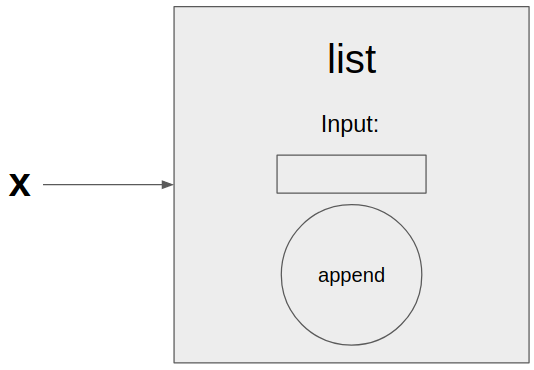
\includegraphics[width=\textwidth]{objectref1.png}
	
	\pause
	
	\column{0.4\textwidth}
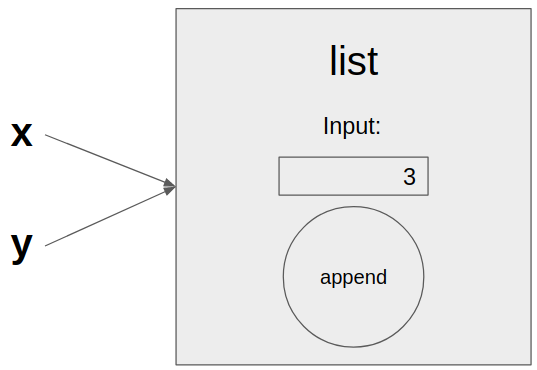
\includegraphics[width=\textwidth]{objectref2.png}
\end{columns}

\end{frame}

\begin{frame}[fragile]{Objekter og metoder}
Det var bl.a. tilfældet med lister:

\begin{columns}
	\column{0.4\textwidth}
	\begin{lstlisting}[style=python]
x = [1,2]
y = x
print(y)
x.append(3)
print(y)
	\end{lstlisting}
	
	\pause
	
	\column{0.4\textwidth}
	\begin{lstlisting}[style=python]
[1, 2]
[1, 2, 3]
	\end{lstlisting}
	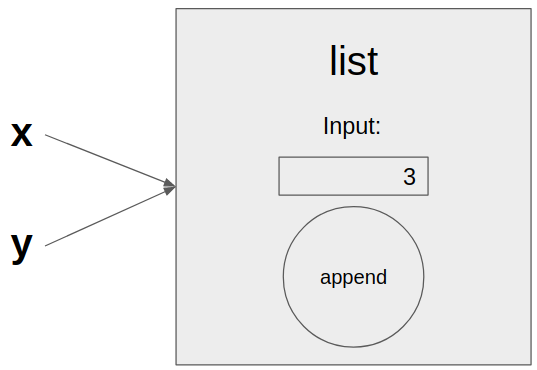
\includegraphics[width=\textwidth]{objectref2.png}
	
\end{columns}

\pause

Hvis det er ved at smelte din hjerne lidt, så husk at det er helt normalt.
\end{frame}

\begin{frame}[fragile]{Objekter og metoder}
Det samme gælder filer.

	\begin{lstlisting}[style=python]
f1 = open("sample_data/README.md", "r")
f2 = f1
print(f1.readline().rstrip())
print(f1.readline().rstrip())
print(f2.readline().rstrip())
f1.close()
	\end{lstlisting}

\end{frame}


\begin{frame}[fragile]{Exceptions}
Hvad sker der hvis vi prøver at læse en fil som ikke eksisterer?

\begin{lstlisting}[style=python]
f = open("fail.txt")
\end{lstlisting}

\pause

\begin{lstlisting}[style=python]
...
FileNotFoundError: [Errno 2] No such file or directory: 'fail.txt'
\end{lstlisting}

Programmet stopper med en fejl!

\end{frame}


\begin{frame}[fragile]{Exceptions}
	Vi kan fange denne fejl (exception), og give en bedre fejlmeddelelse, eller alt efter fejlen prøve at rette op på den.
	
	Dette gøres via \texttt{try} og \texttt{except}:
	\begin{lstlisting}[style=python]
try:
	f = open("fail.txt", "r")
	print(f.read())
	f.close()
except:
	print("Noget gik galt.")
	\end{lstlisting}
\end{frame}

\begin{frame}[fragile]{Exceptions}
	Vi kan også fange en specifik fejl:
	\begin{lstlisting}[style=python]
try:
	f = open("fail.txt", "r")
	print(f.read())
	f.close()
except FileNotFoundError:
	print("Filen kunne ikke findes")
	\end{lstlisting}

\pause

Find den fejltype du ønsker her: 
\url{https://docs.python.org/3/library/exceptions.html}
\end{frame}


\begin{frame}[fragile]{En anden måde at håndtere filer}
Vi kan slippe for at tænke på at lukke filen med et \texttt{with} statement.

\begin{lstlisting}[style=python]
with open("sample_data/README.md", "r") as f:
  for line in f:
    print(line.rstrip())
\end{lstlisting}

\end{frame}

\begin{frame}[fragile]{En anden måde at håndtere filer}
Vi skal dog stadig fange fejl, hvis de opstår:

\begin{lstlisting}[style=python]
try:
	with open("fail.txt", "r") as f:
		for line in f:
			print(line.rstrip())
except:
	print("Noget gik galt.")
\end{lstlisting}

\end{frame}


\begin{frame}[fragile]{Hvad har vi lært?}

\begin{itemize}
	\item Dictionaries
	\item Metoder på dictionaries
	\item Læse fra filer
	\item Skrive til filer
	\item Fange og håndtere fejl
\end{itemize}

Hvilket i princippet er mere end rigeligt til at kunne gøre "alt".


\end{frame}
%
%\begin{frame}[fragile]{Afsluttende bemærkning}
%I har nu lært om bl.a.
%\begin{itemize}
%	\item Typer \& variabler
%	\item If-sætninger
%	\item Funktioner
%	\item Lister
%	\item Løkker
%	\item Strenge
%	\item Dictionaries
%	\item Filer
%\end{itemize}
%
%Hvilket i princippet er mere end rigeligt til at kunne gøre "alt".
%
%
%\end{frame}
%
%
%
%\begin{frame}[fragile]{Afsluttende bemærkning}
%Det vigtigste vi ikke har lært om er hvordan man laver sine egne "klasser", sine egne typer.
%
%\pause
%
%Derudover er der masser af detaljer om de ting vi har lært som også kan udforskes.
%
%\pause
%
%Læs andres kode, læs bøger, se videoer, lav tutorials, lav et projekt og find hjælp på nettet.
%
%\end{frame}

\end{document}